\chapter{Report}

\section{Description of the game}
The name of the Game is “COVID Combat”. It is a 2D game. There is a battlefield consisting of empty places and obstacles through which the active objects (Player and Enemies) of the game can walk and interact. The Player of the Game has an unlimited supply of bullets using which he can kill the enemies. On the other hand, enemies walk randomly and if the Player comes in contact with some enemy, the game is over. If all the enemies are killed, Player wins the game.

\section{What have we achieved TODO}
1.	Grid for the playground has been made.
2.	The Player and Coronaviruses have been added but their behaviours are not yet fully functional.
3.	Sound effects (for background music and player move) have been added.

4. Collision detection between Player and Coronavirus, Shooting Bullets by the Player, Collision Detection between Bullet and Coronavirus.


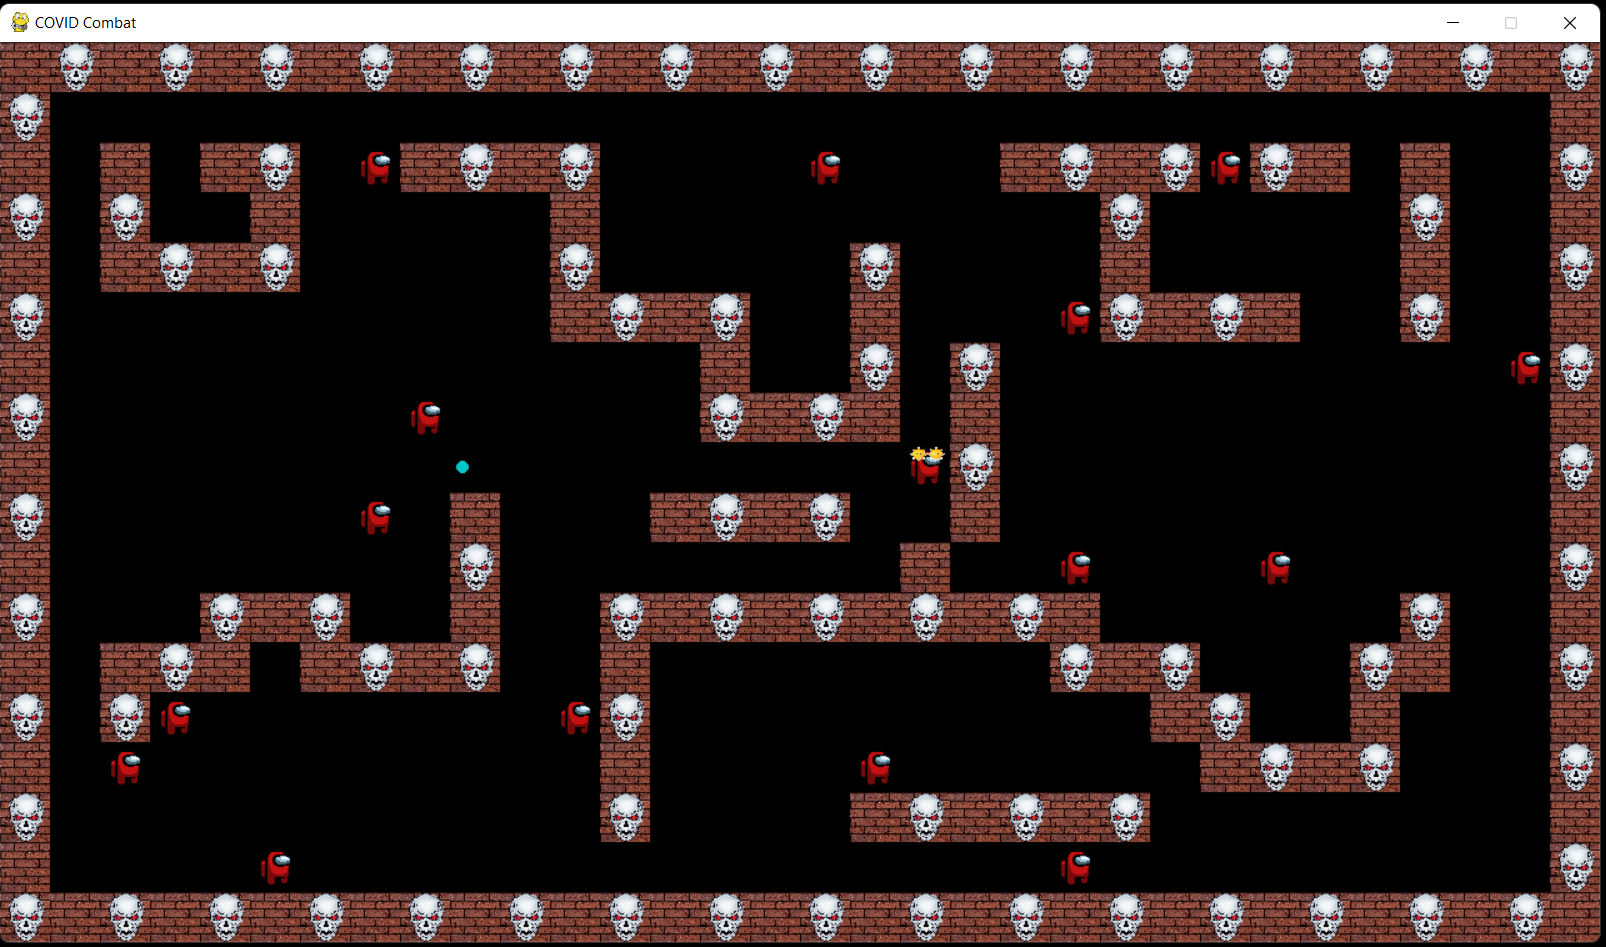
\includegraphics[scale=0.2]{snapshot}

\section{Future Work}
In $Camera.py$ we've some experimental code using which we can cast the 2D grid as a 3D scene and convert this game to a pseudo-3D game. We can add other objects such as sky, floor, hills, trees etc. to make the game look better. Also, we can replace the Player and Enemy images by some realistic characters.

\section{Documentation TODO}
Technologies Used: Python and Pygame for coding the logic
Latex for creating user manual/documentation for the game
HTML/CSS for updating the status of the development.

Code structure is as follows:
\begin{itemize}
  \item main.py - 
      \begin{enumerate}
      \item This imports the necessary python files, and also initiates the main function.
  \end{enumerate}
  \item COVID\_combat.py 
      \begin{enumerate}
      \item Initializes the pygame module
      \item run() initializes the enemy position and direction
      \item run() also keeps on checking for user inputs (arrow keys)
      \end{enumerate}
  \item Battlefield.py
    \begin{enumerate}
      \item draw the grid array by intializing a array
      \item render\_2d\_grid() draws the grids on the canvas
      \end{enumerate}
   \item Player.py
    \begin{enumerate}
      \item update(enemies) - updates the bullet positions and checks collision between bullet and enemies. Based on collision check, enemies are set to dead if required
      \item change\_position(delta\_position) - updates player position based on the arrow key clicked.If new position contains an obstacle, position is not updated.
     \item shoot() - shoots a bullet in the direction in which Player is standing.
     \item rotate\_viewpoint() -- rotates the field of vision of the Player based on mouse events.This will be used in the 3D version of the game.
      \end{enumerate}
    \item Enemy.py
    \begin{enumerate}
      \item update() - updates position based on random movement. Also checks wall collisions
      \end{enumerate}
    \item Camera.py
    \begin{enumerate}
      \item take\_snapshot() -- The camera at the player's position casts rays to the objects in front of the player within field of vision.

      \end{enumerate}
  
\end{itemize}

\section{Running Instructions}
To run this game, you need $python3$ and $pygame$. Installation instructions for $python3$ can be found in $www.python.org$ and for $pygame$ in $www.pygame.org$. Once installed, the game can be run by invoking $python main.py$ from the root directory.